\documentclass[12pt]{article}
%Gummi|065|=)
\usepackage{amsmath, amsfonts, amssymb}
\usepackage[margin=0.5in]{geometry}
\usepackage{xcolor}
%\usepackage{graphicx}
%\usepackage{graphicx}
\newcommand{\off}[1]{}
\DeclareMathSizes{20}{30}{21}{18}

\newcommand{\myhrule}{}

\newcommand{\two }{\sqrt[3]{2}}
\newcommand{\four}{\sqrt[3]{4}}

\newcommand{\dash}{
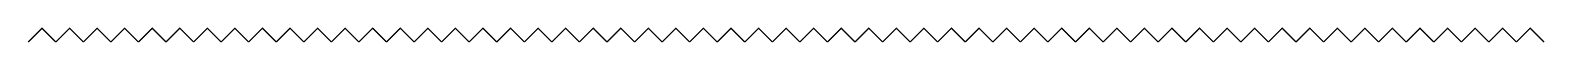
\begin{tikzpicture}[scale=0.35]
\foreach \x in {1,...,55}{
	\draw (\x,-0.25)--(\x+0.5,0.25)--(\x+1,-0.25);
}
\end{tikzpicture}
}

\newcommand{\sq}[3]{
\node at (#1+0.5,#2+0.5) {#3};
\draw (#1+0,#2+0)--(#1+1,#2+0)--(#1+1,#2+1)--(#1+0,#2+1)--cycle;
}

\usepackage{tikz}

\title{\textbf{ Prime Number Theorem: A Conclusion}}
\author{John D Mangual}
\date{}
\begin{document}

\fontfamily{qag}\selectfont \fontsize{25}{30}\selectfont

\maketitle

\noindent Let $G = SU(n)$ be a lie grou and $\mathfrak{g} = \mathfrak{su}(n)$ be the Lie algebra.  I am trying to "evaluate" the product:

$$ \Delta = \prod_{\alpha \in \mathfrak{R}_+} 2 \sin \left( \frac{i\alpha}{2} \right)$$
as described in the first page of this paper by Gukov and Pei.\\ \\
* $\mathfrak{R}_+$ is th set of positive roots of $\mathfrak{g}$ \\ \\
Then is the above product finite?  Aren't roots vectors?  So what does it mean to take $\sin \alpha$ ? \\ \\
* The positive roots are indexed by $0 < j < k < n$ and take diagonal matrices to complex numbers:
$$ \alpha_{jk} : \left[\begin{array}{cccc}
\lambda_1 & & & \\
& \lambda_2 & & \\ 
& & \dots & \\
& & & \lambda_n \end{array}\right] \mapsto (\lambda_j - \lambda_k) $$
Then if $f = \mathrm{diag}(\lambda_1, \dots, \lambda_n) \in (S^1)^{n-1}$ is just such a diagonal matrix the product they are discribing is just the Vandermonde matrix:
$$ \Delta (f)  = \left[\prod_{\alpha \in \mathfrak{R}_+} 2 \sin \left( \frac{i\alpha}{2} \right) \right](f)
= \prod_{j < k} 2 \sin \left( \frac{i(\lambda_i - \lambda_j)}{2} \right)  $$
That looks like Vandermonde matrix.  They define:
$$ \theta(f) = \frac{\Delta (f)^2}{|F|}$$
where $|F|$ counts the kernel:
$$ F = \mathrm{ker}\bigg[ \xi \mapsto \big( \eta \mapsto e^{(n+k)\langle \zeta, \eta \rangle} \big) \bigg] \stackrel{?}{=} \{ 0 \}$$
$F \subseteq T \simeq U(1)^{n-1}$ does not depend on choice of diagonal matrix $f \in T $.  And I think $|F| =1$. \newpage \noindent Multiplication by $(n+k)$ would mean that $0$ would have $n+k$ pre-images and $(n+k)^n$ pre-images on the maximal torus.  \\ \\ What a complicated object!

\newpage

\fontfamily{qag}\selectfont \fontsize{12}{10}\selectfont


\begin{thebibliography}{}

\item J{\o}rgen Ellegaard Andersen, Sergei Gukov, Du Pei \textbf{The Verlinde formula for Higgs bundles} \texttt{arXiv:1608.01761}





\end{thebibliography}



\end{document}